\documentclass[main.tex]{subfiles}
\graphicspath{{pictures/}}
\begin{document}

\section{Software system design}

The main goals for the software system was the following:
\begin{enumerate}
    \item To separate safety critical and non-safety critical code as much as possible.
    \item Building the non safety critical part to be easily extended and changed without needing to even recompile other parts.
    \item Build the safety critical part as robust as possible by regarding it as a hard real time system.
\end{enumerate}


To begin with we had the software system from last years project (?ref?).
After further examination it was clear that to be able to reach the goals the whole software system
needed to be redesigned and rewritten. A design fulfilling the goals is presented in this section.
First what the big parts are and how the fit together is described in the overview (section \ref{sec:sw_design_overview}),
after this the design of each part is described in detail.

\subsection{Overview}
\label{sec:sw_design_overview}

\begin{figure}[H]
    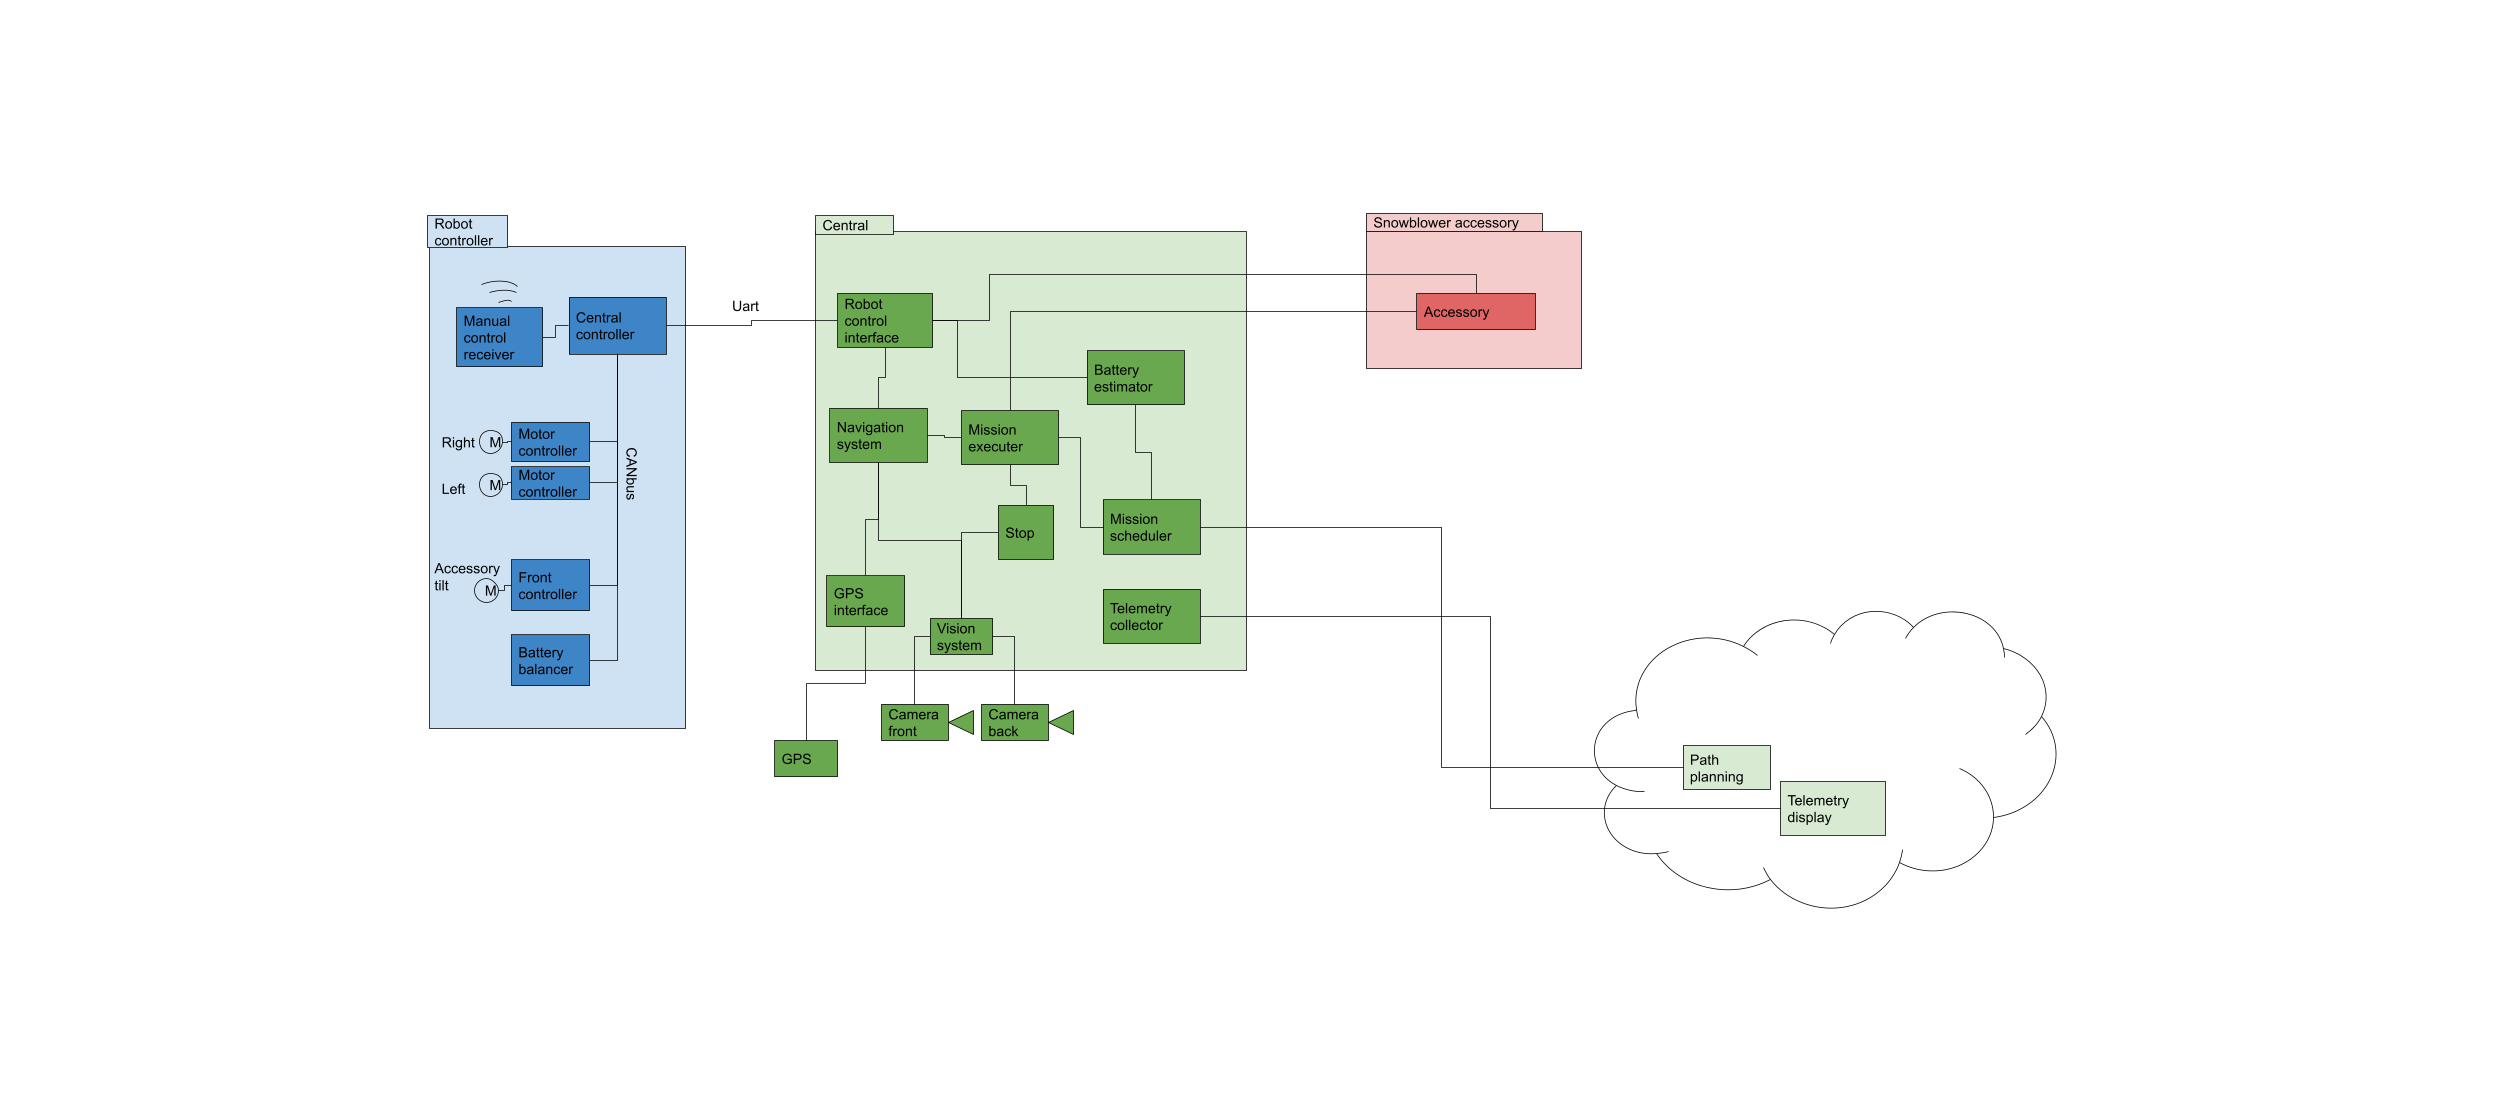
\includegraphics[width=\textwidth]{software_overview.png}
    \caption{Overview of the software architecture.}
    \label{fig:software_overview}
\end{figure}

The design of the software system is made up of different parts and are shown in figure \ref{fig:software_overview}. 
In figure \ref{fig:software_overview} each system is symbolized by a square with a describing name and
lines symbolize communication between systems. Some communication lines are omitted for clarity, what other system each system communicates with is described in the more detailed description of the system design.

The design was divided into 4 main parts, each part has its own color in figure \ref{fig:software_overview}:

The safety critical part is shown in blue and controls the robot directly. 
It's made up of mikrocontrollers running custom firmware written in rust using the RTIC framework (?ref?) except
for the motor controllers that run the Vesc firmware (?ref?).
This systems in this part communicate with each other using one single shared CANbus and communicate with all other systems over a UART link to the robotcontroller interface.

The non safety critical part is shown in the green big rectangle.
This part handles everything needed to do to carry out a mission and sends the proper commands to either the robot controller or the accessory. This part is made up of many interchangeable systems orchestrated in a Arrowhead local cloud (?ref?).

The red part is the accessory, it controls the accessory directly and is a system in the local cloud.
The accessory is designed to be able to be any kind of accessory. In out test case it is a snowblower.

The last part in light green in the little cloud is a separate Arrowhead local cloud running on a server somewhere. It is designed to be the interface between the robot and the world being able to get telemetry from the robot and send missions for it to do.

\subsection{Design of all the parts}

\subsubsection{Mission scheduler}

\subsubsection{Mission executor}

\end{document}